\section{If-statements}

\subsection*{internal explanation}

The exercises let the students build programs themselves using if-statements. Each program is based on building up the rules of a game. They will be given cards where they can build each rule of the game they are working with. 

\begin{figure}[H]
    \makebox[\textwidth][c]{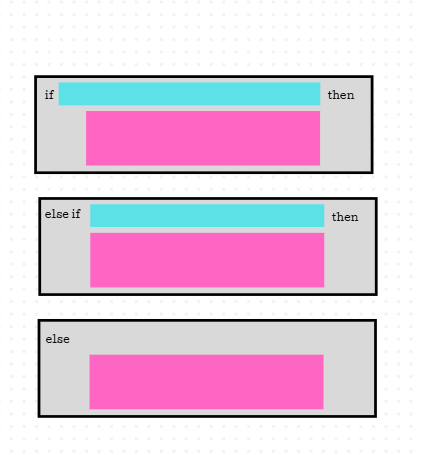
\includegraphics[width=0.5\linewidth]{Billeder/if cards.png}}
    \caption{if statements}
\end{figure}

They will have to attach keywords to the cards using velcro. The conditions for each rule should be in the blue box, and the rest should be in the pink box. 


\begin{figure}[H]
    \makebox[\textwidth][c]{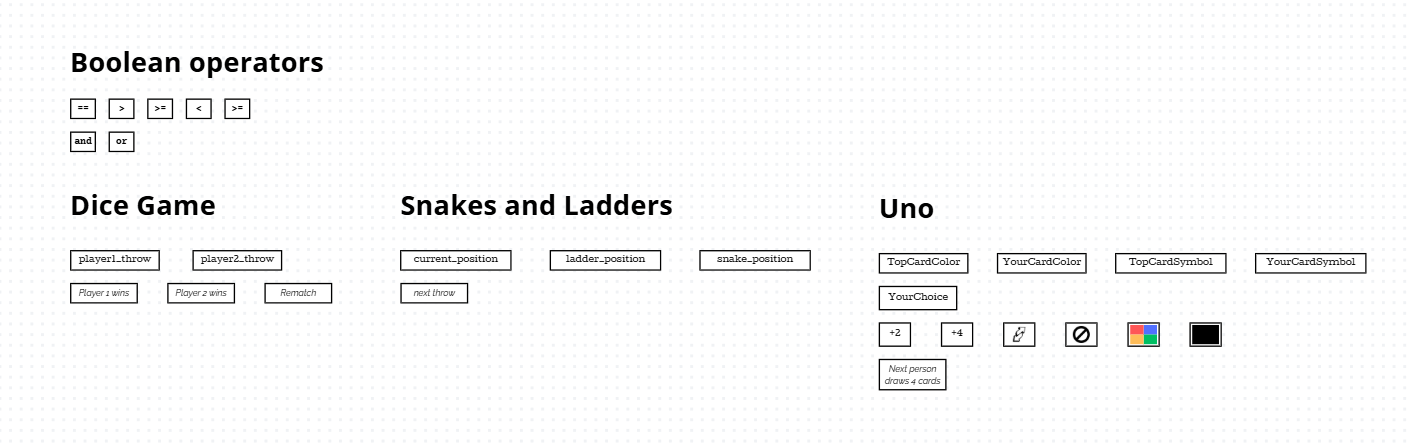
\includegraphics[width=1\linewidth]{Billeder/if keywords.png}}
    \caption{if statements}
\end{figure}

Examples of correct programs for each game can be seen below, but the students can build as many rules as they want. Each card can contain a rule and then they can arrange the cards to make a program. 


There are also bigger cards for nested if statements. Remember every condition containing "and" can be converted to a nested if-statement and every condition containing "or" can be converted to "else if". 

The students can place the smaller cards inside the bigger cards to make nested if-statements.

\begin{figure}[H]
    \makebox[\textwidth][c]{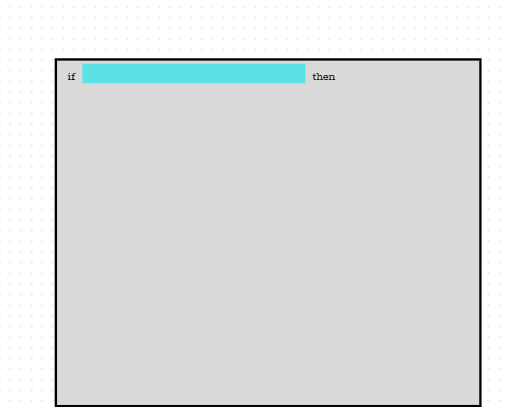
\includegraphics[width=0.5\linewidth]{Billeder/bigger if cards.png}}
    \caption{if statements}
\end{figure}

There are also cards for bigger conditions

\begin{figure}[H]
    \makebox[\textwidth][c]{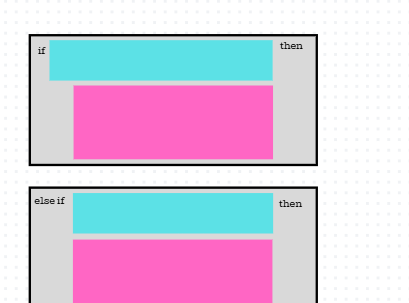
\includegraphics[width=0.5\linewidth]{Billeder/fat condition vards.png}}
    \caption{if statements}
\end{figure}









You can think of an if-statement as a question: if the answer is “yes,” the condition is true and the computer runs the specified command; if the answer is “no,” it skips to the next command. You can use it if you want to be able to generalize your code to handle different cases or exceptions. The goal of your program may for example depend on what the user asks for, or how much input is received. 

\subsection*{Materials}

\begin{itemize}
    \item[-] Markers
    \item[-] Laminated Exercises
    \item[-] Dices
\end{itemize}

\subsection*{To Do}
\begin{itemize}
    \item[-] Make cheat sheet (Uno)
    \item[-] Laminate Cheat sheet and exercises
\end{itemize}


\subsection*{Exercises}

\subsection*{Dice Game}

\textbf{Dice game rules}: two people throw a dice and the biggest number wins. In case of a tie you repeat it. 



Options:

\begin{itemize}
\color{red}
\item if
\item else 
\item else if
\end{itemize}

\begin{itemize}
\color{CornflowerBlue}
\item > (greater than)
\item >= (greater than or equal to)
\item < (less than)
\item <= (less than or equal to)
\item == (equal to)
\end{itemize}

\vspace{1cm}
\textcolor{red}{\rule[-0.5ex]{0.7cm}{1pt}} my\_throw \textcolor{CornflowerBlue}{\rule[-0.5ex]{0.7cm}{1pt}} your\_throw then

\hspace{1cm} \textit{I win}

\textcolor{red}{\rule[-0.5ex]{0.7cm}{1pt}} my\_throw \textcolor{CornflowerBlue}{\rule[-0.5ex]{0.7cm}{1pt}} your\_throw then

\hspace{1cm} \textit{I lose}

\textcolor{red}{\rule[-0.5ex]{0.7cm}{1pt}}

\hspace{1cm} \textit{rematch}

\textbf{Solution:}

\textcolor{red}{if} my\_throw \textcolor{CornflowerBlue}{>} your\_throw then

\hspace{1cm} \textit{I win}

\textcolor{red}{else if} my throw \textcolor{CornflowerBlue}{<} your throw:

\hspace{1cm} \textit{I lose}

\textcolor{red}{else:}

\hspace{1cm} \textit{rematch}







\subsection*{Snakes and Ladders}


\begin{figure}[H]
    \makebox[\textwidth][c]{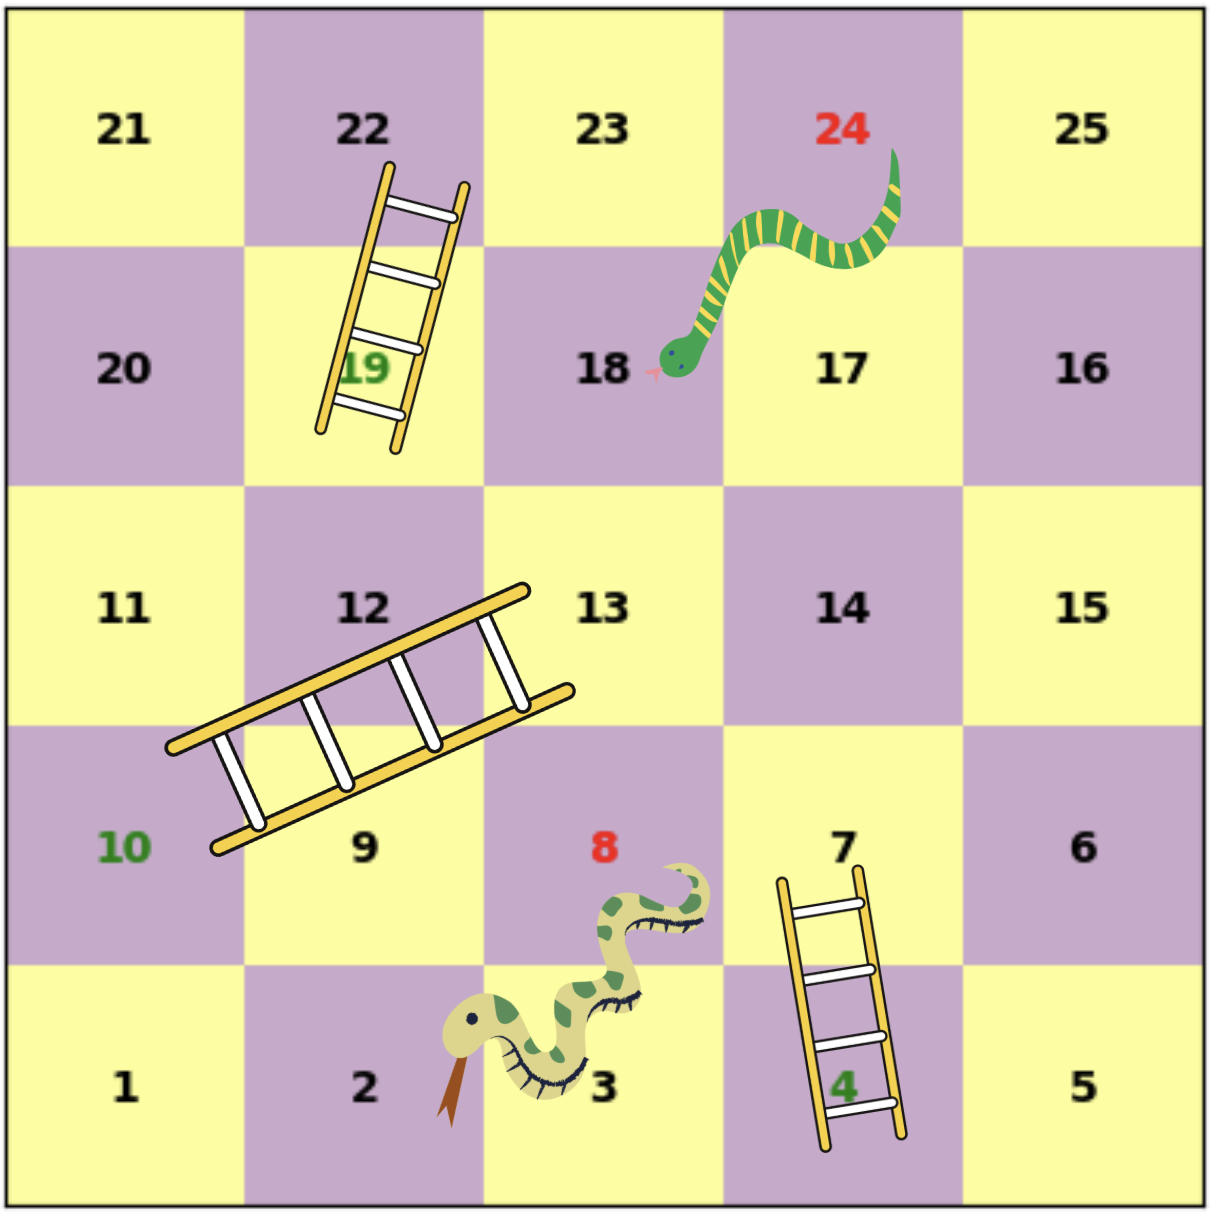
\includegraphics[width=1\linewidth]{Billeder/SnakesLadders.png}}
    \caption{Snakes and Ladders}
\end{figure}


\textbf{Exercise:}

Options:

\begin{itemize}
\color{red}
\item if
\item else 
\item else if
\end{itemize}

\begin{itemize}
\color{CornflowerBlue}
\item > (greater than)
\item >= (greater than or equal to)
\item < (less than)
\item <= (less than or equal to)
\item == (equal to)
\end{itemize}

\begin{itemize}
\color{Plum}
\item *insert number*
\end{itemize}

\vspace{1cm}

current\_position = current\_position + eyes 

\hspace{0.1cm}


\textcolor{red}{\rule[-0.5ex]{0.7cm}{1pt}} current\_position \textcolor{CornflowerBlue}{\rule[-0.5ex]{0.7cm}{1pt}} ladder\_position then

\hspace{1cm} 
current\_position = current\_position + \textcolor{Plum}{\rule[-0.5ex]{0.7cm}{1pt}}

\hspace{0.1cm}

\textcolor{red}{\rule[-0.5ex]{0.7cm}{1pt}} current \_position \textcolor{CornflowerBlue}{\rule[-0.5ex]{0.7cm}{1pt}} snake\_position then 

\hspace{1cm} current\_position = current\_position - \textcolor{Plum}{\rule[-0.5ex]{0.7cm}{1pt}}

\textit{next throw}

\vspace{1cm}

\textbf{Solution:}


current\_position = current\_position + eyes 

\hspace{0.1cm}


\textcolor{red}{if} current position \textcolor{CornflowerBlue}{==} ladder\_position: 

\hspace{1cm} 
current\_position = current\_position + \textcolor{Plum}{3}

\hspace{0.1cm}

\textcolor{red}{else if} current \_position \textcolor{CornflowerBlue}{==} snake\_position: 

\hspace{1cm} current\_position = current\_position - \textcolor{Plum}{6}

\textit{next throw}


\subsection*{Uno}

\textbf{Exercise:}

Options:

\begin{itemize}
\color{red}
\item if
\item else 
\item else if
\end{itemize}

\begin{itemize}
\color{CornflowerBlue}
\item > (greater than)
\item >= (greater than or equal to)
\item < (less than)
\item <= (less than or equal to)
\item == (equal to)
\end{itemize}

\begin{itemize}
\color{LimeGreen}
\item and   
\item or
\end{itemize}



\textcolor{red}{\rule[-0.5ex]{0.7cm}{1pt}} your\_card\_color \textcolor{CornflowerBlue}{\rule[-0.5ex]{0.7cm}{1pt}} top \_card\_color \textcolor{LimeGreen}{\rule[-0.5ex]{0.7cm}{1pt}}
your\_card\_symbol \textcolor{CornflowerBlue}{\rule[-0.5ex]{0.7cm}{1pt}}
top\_card\_symbol:

\hspace{1cm}
top\_card\_color=your\_card\_color

\hspace{1cm}
top\_card\_symbol=your\_card\_symbol

\textcolor{red}{\rule[-0.5ex]{0.7cm}{1pt}} 
your\_card\_color \textcolor{CornflowerBlue}{\rule[-0.5ex]{0.7cm}{1pt}} black:

\hspace{1cm}
\textcolor{red}{\rule[-0.5ex]{0.7cm}{1pt}} your\_card\_symbol \textcolor{CornflowerBlue}{\rule[-0.5ex]{0.7cm}{1pt}} "+4":

\hspace{2cm} top\_card\_color = your\_choice

\hspace{2cm}
top\_card\_symbol=Any

\hspace{2cm}
\textit{next person draws 4 cards}

\hspace{1cm}
\textcolor{red}{\rule[-0.5ex]{0.7cm}{1pt}:}

\hspace{2cm}
top\_card\_color=your\_choice

\hspace{2cm}
top\_card\_symbol=Any

\textcolor{red}{\rule[-0.5ex]{0.7cm}{1pt}:}

\hspace{1cm}
\textit{Draw a card}

\vspace{1cm}

\textbf{solution:}



\textcolor{red}{if} your\_card\_color \textcolor{CornflowerBlue}{==} top \_card\_color \textcolor{LimeGreen}{or}
your\_card\_symbol \textcolor{CornflowerBlue}{==}
top\_card\_symbol:

\hspace{1cm}
top\_card\_color=your\_card\_color

\hspace{1cm}
top\_card\_symbol=your\_card\_symbol

\textcolor{red}{else if} 
your\_card\_color \textcolor{CornflowerBlue}{==} black:

\hspace{1cm}
\textcolor{red}{if} your\_card\_symbol \textcolor{CornflowerBlue}{==} "+4":

\hspace{2cm} top\_card\_color = your\_choice

\hspace{2cm}
top\_card\_symbol=Any

\hspace{2cm}
\textit{next person draws 4 cards}

\hspace{1cm}
\textcolor{red}{else:}

\hspace{2cm}
top\_card\_color=your\_choice

\hspace{2cm}
top\_card\_symbol=Any

\textcolor{red}{else:}

\hspace{1cm}
\textit{Draw a card}












